% document settings
\documentclass[a4paper, openany]{book}
\usepackage{amsmath, amsthm, amssymb, graphicx}
\usepackage{geometry,fontspec, xeCJK, indentfirst}

% document layout and style settings
\usepackage[bookmarks=true, colorlinks, citecolor=blue, linkcolor=black]{hyperref}
\usepackage{amsmath, cleveref, caption, subcaption}
\usepackage[T1]{fontenc}
\usepackage{textcomp}
\geometry{a4paper, scale = 0.8}
\setmainfont{Noto Serif}
\setsansfont{Noto Sans}
\setmonofont{Noto Sans Mono}
%\setCJKmainfont{Noto Serif SC}
%\setCJKsansfont{Noto Sans SC}
\setlength{\parindent}{2em}
\captionsetup{format = hang, font = small, labelfont = bf, labelsep = quad}

% metadata
\title{Note for Computational Analysis}
\author{Zhen-Lin Huo}
\date{\today}

% document content
\begin{document}

\maketitle
\frontmatter
\tableofcontents

% main content starts from here
\mainmatter

Generative Design = Computational Analysis + Computational Synthesis

Computational Analysis: More on rule than result

\chapter{Information Theory}

\begin{quote}
The only way to rectify our reasoning is to make them as tangible as those of the Mathematicians, so that we can find our error at a glance, and when there are disputes among persons, we can simply say: Let us calculate (calculemus), without further ado, to see who is right.
  \begin{flushright}
    --- Leibniz, The Art of Discovery (1685)
  \end{flushright}
\end{quote}

\section{Formal Language}

Use a set of arbitrary symbols and rules for manipulating them

\begin{itemize}
  \item Have Syntax
  \item Not Semantics (no meanings)
\end{itemize}

\section{Finite State Machine}

A theoretical computing machine

Alan Truing

\begin{itemize}
  \item The machine can be in one of a finite number of states
  \item Can change (academically, \emph{transit}) from one state to another in
  response to some inputs
\end{itemize}

\subsection{Turing Machine}

Alan Turing (1936)

\begin{itemize}
  \item A tape
  \begin{itemize}
    \item Has infinite length
    \item Is divided into cells
    \item Is blank, or contain a symbol
  \end{itemize}
  \item The head
  \begin{itemize}
    \item Can read/write/erase
    \item Can move left/right
  \end{itemize}
  \item State Register
  \begin{itemize}
    \item Machine can be one a number of states
  \end{itemize}
  \item Transition Table
  \begin{itemize}
    \item Erase/Write a symbol
    \item Move the head (L/R)
    \item Change machine state
  \end{itemize}
\end{itemize}

\subsection{Universal Turing Machine}

Universal Turing Machine~simulates a Turing Machine. It contains a
Turing Machine description as input along with an input string, runs the
Turing Machine on the input and returns a result.

Turning Machine + Encoded Type (Programme) = Universal Turing Machine

\subsection{Markov Model}

\begin{itemize}
  \item have a finite set of states
  \item different states (or group of states) have different probabilities to
  turn into other states (or itself)
\end{itemize}

If add memory into the Markov Model, we can get a second-order Markov
Model (dependent on (t-1) and (t))

The system will look different depending on how the states are defined.

\section{Information}

\subsection{Uncertainty}

\textbf{Entropy} 熵

Entropy of X is the amount of uncertainty in X

\emph{associated with X}

entropy = information

Quantify:

\begin{itemize}
  \item \(S = \mathit{k} \log W\) (Boltzmann)
  \item \(H ( X ) = -\sum_{\mathit{x}\in X}^{} p ( \mathit{x} ) \log p ( \mathit{x} )\)
\end{itemize}

\subsection{Shannon-Fano Coding (Fano's
Method)}

In a piece of given information (e.g.~a sentence):

\begin{enumerate}
  \item Calculate the frequency of each character
  \item Divide the characters into two groups (0 and 1) based on their
  frequencies
  \begin{itemize}
    \item make each group has approximately 50\% of the total frequency
  \end{itemize}
  \item Repeat the process to that 2 groups, until each group has only one
  character
\end{enumerate}

Actual entropy of given message:

\[H ( X ) = -\sum_{\mathit{x}\in X}^{} p ( \mathit{x} ) \log p ( \mathit{x} )\]

Mean word length:

\[E\left [ \mathit{I} ( \mathit{x} )  \right ] =  \sum_{\mathit{x}\in X}^{} p ( \mathit{x} ) Level\]

\subsection{Communication}

\textbf{Mutual Information}

\[\mathit{I} ( \mathit{X}; \mathit{Y} ) = \mathit{H} ( \mathit{Y} ) - \mathit{H} ( \mathit{Y} \mid \mathit{X} )\]

\textbf{Channel Capacity}

\[\max_{\mathit{f}} \mathit{I} ( \mathit{X}; \mathit{Y} )\]

Channel capacity is determined by:

\begin{itemize}
  \item Message coding
  \item Noise
\end{itemize}

\section{Formalising Natural Language}

\subsection{Pure Syntax}

\subsubsection{Finite State (Markov) Grammar}\label{FSM-Grammar}

Treat each word as a state, then a sentence can be constructed by a Markov Process.

\emph{1\textsuperscript{st} order}

\begin{figure}[htbp]
  \centering

  \parbox[t]{0.29\textwidth}{The man comes

    The men come}
  \begin{subfigure}{0.39\textwidth}
    \raggedright
    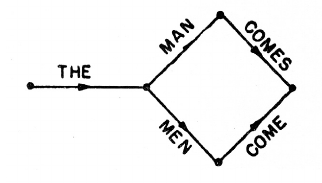
\includegraphics[width=0.5\textwidth]{../assets/MarkovGrammar1.png}
  \end{subfigure}
\end{figure}

or

\begin{figure}[htbp]
  \centering
  \parbox[t]{0.29\textwidth}{The old man comes

    The old men come}
  \begin{subfigure}{0.39\textwidth}
    \raggedright
    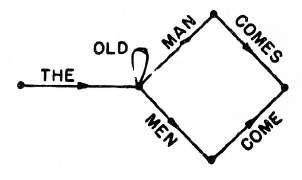
\includegraphics[width=0.5\textwidth]{../assets/MarkovGrammar2.png}
  \end{subfigure}
\end{figure}

No memory $\rightarrow$ Cannot solve complex order

\emph{n\textsuperscript{th} order}

\begin{quote}
  The old man I met last week comes

  The old men I met last week come
\end{quote}

\subsubsection{Chomsky (1957): Grammar as Recursive
Rules}

\begin{itemize}
  \item S $\rightarrow$ NP + VP
  \item NP $\rightarrow$ N + auxP
\end{itemize}

\begin{figure}[htbp]
  \centering
  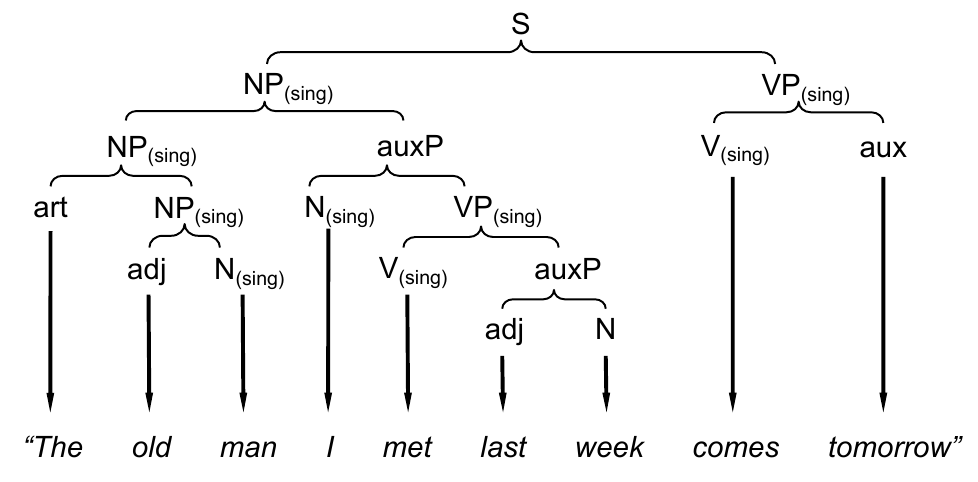
\includegraphics[width=0.8\textwidth]{../assets/GrammarAsRecursiveRules1.png}
\end{figure}

\subsection{Computer Cognition}

\subsubsection{Turing Test}

Recognising intelligence: how to evaluate whether a computer has intelligence?

Alan Turing (1949), the imitation game:

\begin{itemize}
  \item A man (\textbf{A}) in a room, communicating with another man (\textbf{C}) with text
  \item A computer (\textbf{B}) in the same room, communicating with (\textbf{C})
  \item If \textbf{C} cannot distinguish \textbf{B} as a computer or a human, then \textbf{B} is intelligent
\end{itemize}

\subsubsection{ELIZA (1665)}

A Computer Programme for the Study of Natural Language Communication between Man and Machine

\begin{flushright}
  ---Joseph Weizenbaum, 1966
\end{flushright}

\begin{itemize}
  \item Pick some key words from human reply, and ask questions about these words.
  \item ``Simulating intelligence''
\end{itemize}

\subsubsection{Searle's ``Chinese Room'' (1980)}

Extension of Turing Test:

\begin{itemize}
  \item Searle is the one in the room, and he doesn't understand Chinese
  \item a series of instructions are given to Searle, telling him what to reply when seeing different messages.
  \item Outer people cannot tell whether Searle himself understand  Chinese or not
\end{itemize}

\textbf{Dualism in The Mind}

The Chinese Room argument split language into \textbf{syntax} (rules in the instructions) and \textbf{semantics} (understanding the meaning of the words in mind).

It suppose: A symbolic (mental) level must be essentially arbitrary and meaningless and it maps easily onto the real world.

\section{The Limits of Formal Systems}

\subsection{Characteristica Universalis}

Firstly proposed by Gottfried Leibniz in 17\textsuperscript{th} century.

An idea for a /textbf{universal symbolic language} --- especially in /textbf{logic, mathematics, science, and philosophy}. Leibniz believed that if we could reduce reasoning to a kind of calculation using symbols, then disagreements could be resolved by computation, like solving an equation.

\subsubsection{Construction of \textit{Characteristica Universalis}}

\begin{itemize}
  \item \textbf{Symbols for Concepts}: For every basic idea of concept
  \item \textbf{Combinatorial Rules}: Complex ideas would be built by combining simpler ones, using logical and mathematical rules—similar to how algebra or programming languages work.
  \item \textbf{Logical Structure}: Tightly connected to \textbf{formal logic}, so reasoning could be done mechanically just like a machine, following steps.
  \item \textbf{Inspired by Mathematics}: As precise and unambiguous as mathematics, so that can avoid the vagueness of natural languages.
\end{itemize}

\subsubsection{David Hilbert (1900): Attempt to Complete It}

23 problems (to be resolved by 20\textsuperscript{th} century mathematics)

\subsection{Kurt Gödel}

\subsubsection{Gödel's Incompleteness Theorems (1931)}

\begin{quote}
  For every $\omega$-consistent recursive class $\kappa$ of formulas, there are recursive class signs $\mathsf{r}$ such that neither $\forall \mathsf{vr}$ nor $\neg \forall \mathsf{vr}$ is in $\kappa$.
\end{quote}

This means, in a consistent formal system, there are always some true statements that cannot be proved within that system. 

\begin{quote}
  e.g.
  \begin{enumerate}
    \item Sentence \# 2 is true.
    \item Sentence \# 1 is false.
  \end{enumerate}

  And\dots

  There exists no proof of this statement.
\end{quote}

\subsubsection{About Formal System}

Gödel described a way to number a formal system. e.g.

\hspace*{\fill}

\begin{tabular}{ccl}
  Sign & Gödel \# & Meaning \\
  \hline
  $\neg$ & 1 & not \\
  $\lor$ & 2 & or \\
  $\supset$ & 3 & if \dots then \\
  $\exists$ & 4 & there exists \\
  $=$ & 5 & equals \\
  $0$ & 6 & zero \\
  $s$ & 7 & immediate successor \\
  $($ & 8 & \\
  $)$ & 9 & \\
  $,$ & 10 & \\
  $+$ & 11 & plus \\
  $\times$ & 12 & times \\
\end{tabular}
\qquad
\begin{tabular}{ccc}
  Sign & Gödel \# & Possible Substitution \\
  \hline
  $x$ & 13 & 0 \\
  $y$ & 14 & s0 \\
  $z$ & 15 & y \\
  $p$ & $13^2$ & $0 = 0$ \\
  $q$ & $17^2$ & $( \exists x ) ( x = sy )$ \\
  $r$ & $19^2$ & $p \supset q$ \\
  $P$ & $13^3$ & $x = sy$ \\
  $Q$ & $17^3$ & $\neg ( x = ss0 \times y )$ \\
  $R$ & $19^3$ & $( \exists z ) ( x = y + sz )$
\end{tabular}

\hspace*{\fill}

\hspace*{\fill}

Then a formal system can be numbered like below:

$$e.g. \  ( \exists x ) ( x = sy )$$

\begin{figure}[htbp]
  \centering
  \includegraphics[width=15em]{../assets/GödelNumber1.png}
\end{figure}

Gödel number of it can be calculated:
$$m = 2^8 \times 3^4 \times 5^{13} \times 7^9 \times 11^8 \times 13^{13} \times 17^5 \times 17^5 \times 19^7 \times 23^{17} \times 29^9$$

Gödel number for sequence of formulas:
$$( \exists x ) ( x = sy ) \  \rightarrow \  m$$
$$( \exists x ) ( x = s0 ) \  \rightarrow \  n$$
$$\mathsf{sequence} \  k = 2^m \times 3^n$$

So that any expression (e.g. formula, proof, etc.) as a Gödel number.

\textbf{\textit{Question: How to understand the relationship between the Gödel number and whether it can be proved?}}

\dots And finally, we can see, in a consistent formal system, there are always some true statements that cannot be proved within that system.

\section{Non-Formal Alternatives}

To conclude, Leibniz proposed the ideal of formalising and formal language, and Gödel proved that the formal systems are limited.

\begin{quote}
  Since man at least adapts (a truism, for any large dynamic system does so) there is no genuine ‘channel capacity’ in Shannon’s (1949) sense. For the load imposed by an input may depend upon all of the inputs received up to the moment in question. Or put commonsensically, as it may be if the subject is assumed to learn input/output relations, a once difficut task will become less difficult as the task relation is learned.

  \begin{flushright}
    --- Pask G, \textit{Communication Cognition and Learning}, 1975
  \end{flushright}
\end{quote}

The language may not be formal, because they showed great ambiguity.

\subsection{Grammatical Structure}\label{FSM-Grammar2}

Think back to Markov Chain and Finite State Machine, we can subdivide the state of a finite state machine, so they can do better than the previous version (\textbf{\cref{FSM-Grammar}}).

\begin{figure}[htbp]
  \centering
  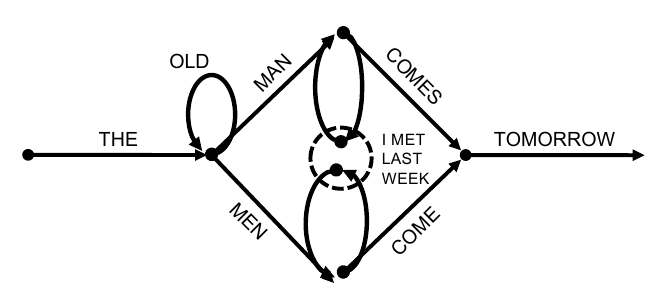
\includegraphics[width=20em]{../assets/GrammaticStructure1.png}
\end{figure}

\subsubsection{Predicting Grammatical Structure (Jeffrey Elman): A Dynamical System}

\paragraph{Neural Network}

The previous mentioned Markov process (\textbf{\cref{FSM-Grammar2}}) can be coded into a neural network:

\begin{quote}
  input unit(s) --- recurrent layer --- output unit(s)
\end{quote}

The recurrent layer can capture changes (word sequence) over time.

After training, this network is able to predict what type of word will come next in a sentence.

In this network, \textbf{syntax} and \textbf{semantics} are in the same space.

\paragraph{Words \& Sentences in High Dimensional Space}

\subparagraph{Convert Words into Vectors}

In this neural network, each word activates neurons in the hidden layer differently, which can be mapped as vectors in a high dimensional space (state space).

A single word will correspond to a series of points in the state space.

\subparagraph{Sentence in State Space}

As a sentence is a sequence of words, constructing a sentence is just connecting different points / vectors in the state space.

The same word with different grammatical context will have similar but not same route in the state space.

\subsection{Computational Design}

In the field of linguistics, the main body of work is about the \textbf{structure rules}, but in the field of design and computer code, question goes to \textbf{processing rules}.

\subsubsection{Design Process: \textit{Exposure} from Antony Gormley}

The design process of this sculpture is moving between processing rules and structure rules (\textbf{\cref{fig:ExposeDesignProcess1}}).

\begin{figure}[htbp]
  \centering
  \begin{subfigure}{0.39\textwidth}
    \centering
    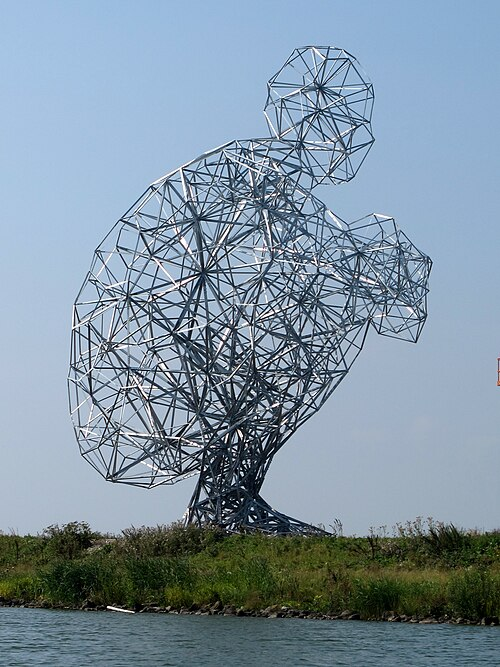
\includegraphics[width=0.6\textwidth]{../assets/Exposure1.jpg}
    \caption{The Scuplture \textit{Exposure} by Antony Gormley}
    \label{fig:Exposure1}
  \end{subfigure}
  \begin{subfigure}{0.59\textwidth}
    \centering
    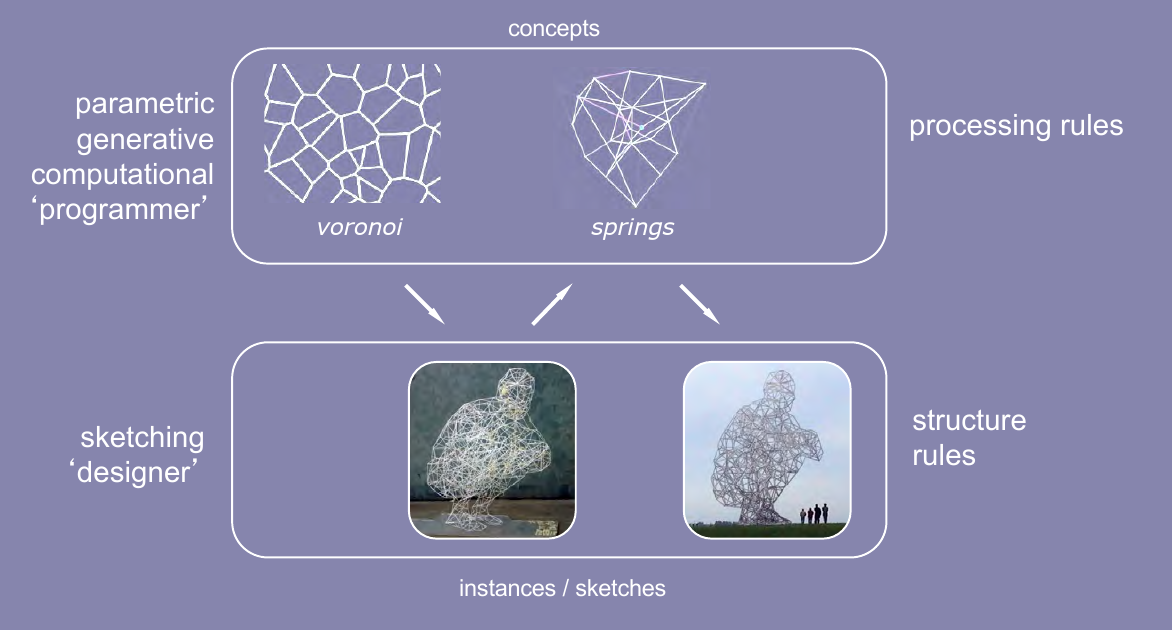
\includegraphics[width=\textwidth]{../assets/ExposureDesignProcess1.png}
    \caption{The Design Process of \textit{Exposure}}
    \label{fig:ExposeDesignProcess1}
  \end{subfigure}
\end{figure}

\subsubsection{``Wicked Problems'' by Rittel \& Webber}

\paragraph{Define Structure \& Define Process}

In the field of design (e.g. architecture, planning, etc.), most problems are unique and not exactly defined. From different point of view, the same problem can be solved differently. There is no right or wrong solution, problems are connected, etc. Such complex problems make the design process cannot predefine the process to find out the solution.

On the other hand, design in automotive, aerospace, ect., are doing optimisation, thus the goal is determined, the process is know and integrated.

Similar compariason can also be made between traditional construction and formal system. The traditional construction is defining structure, with knowledge embedded throughout the whole process, while the formal system is process determined.

\paragraph{Narrow Channels}

Vision: Form 126 million receptors to 140 million neurons via only 1 million nerve fibres.

Design: From orginal design structure to finished construction structure with design communication processing.

\chapter{Space Syntax}

\section{Spatial Structure}

\subsection{Graph Representation of Spacial Configuration}

Space Syntax represent street use topological graph: each street is a node, connect nodes based on their connection relationship.

These analysis is \textbf{probabilistic}, not refers to any individual human behaviour.

\subsubsection{Depth}

Depth means how many street one need to reach to another node.

\subsubsection{Integration}

Means the routes \textit{to} a location.

A node has high integration means it is more likely to be more central, people will tend to reach here.

\subsubsection{Choice}

Means the routes \textit{through} a location, higher choice means it is more frequently appears in the shortest route to other streets, that is people will tend to pass here to other destination.

A node has higher choice means it is more likely to be a path for natural crowd, while one with low choice means it is less likely used for navigation.

\subsubsection{Intelligibility}

Intelligibility means \textbf{how easy it is to find a route} from one location to another.

In more technical terms, intelligibility is quantified as the correlation between \textbf{local connectivity} (how many immediate connections a space has) and \textbf{global integration} (how central a space is within the entire system).

High intelligibility means that local observations provide a good sense of the overall spatial structure, making navigation intuitive. Conversely, low intelligibility suggests that the space is fragmented or difficult to grasp without external information.

\begin{figure}[htbp]
  \centering
  \begin{tabular}{ccl}
    \hline
    \textbf{Integration} & \textbf{Choice} & \textbf{Type of Street}\\
    \hline
    High & High & Town Centre \& Main Street\\
    Low & High & Bridge \& Tunnel\\
    Low & Low & Dead-end Street \& Private Roads\\
    \hline
  \end{tabular}
  \caption{Different types of street in axial analysis}
  \qquad
  \begin{tabular}{cl}
    \hline
    \textbf{Type of Space} & \textbf{Intelligibility}\\
    \hline
    Urban Planning & \textbf{High Intelligibility} \\ & Easier to navigate, fostering pedestrian movement and social interaction\\
    Architectural Design & \textbf{High Intelligibility}\\ & Help understand paths and destinations\\
    Wrokspace & \textbf{Low Intelligibility} \\ (e.g. IKEA) & Create exploratory movement patterns, longer stays, increase engagement\\
    \hline
  \end{tabular}
  \caption{Different types of space need different intelligibility on purpose}
\end{figure}

\subsection{Axial Map Analysis}

Axial map is an abstraction of the space to straight lines, drawn through space, by a formal algorithm. It has been discovered that the graph of the resulting network lines of correlate with general pedestrian movement.

\subsubsection{Angular Analysis}

Dalton introduced angular analysis of axial maps in order to move of how people use minimal angular strategies to navigate from location to location.

\subsubsection{Scale of Observation}

Under different scale of observation, different centre will be identified. And centre in different scale of observations represents functional space in different scale. For example, centre of 500 metre radius may represents to markets (\textbf{\cref{fig:ScaleOfObservation1}}), while centre of 10 kilometres may refer to important functional space of the city (\textbf{\cref{fig:ScaleOfObservation2}}).

\begin{figure}[htbp]
  \centering
  \begin{subfigure}{0.49\textwidth}
    \centering
    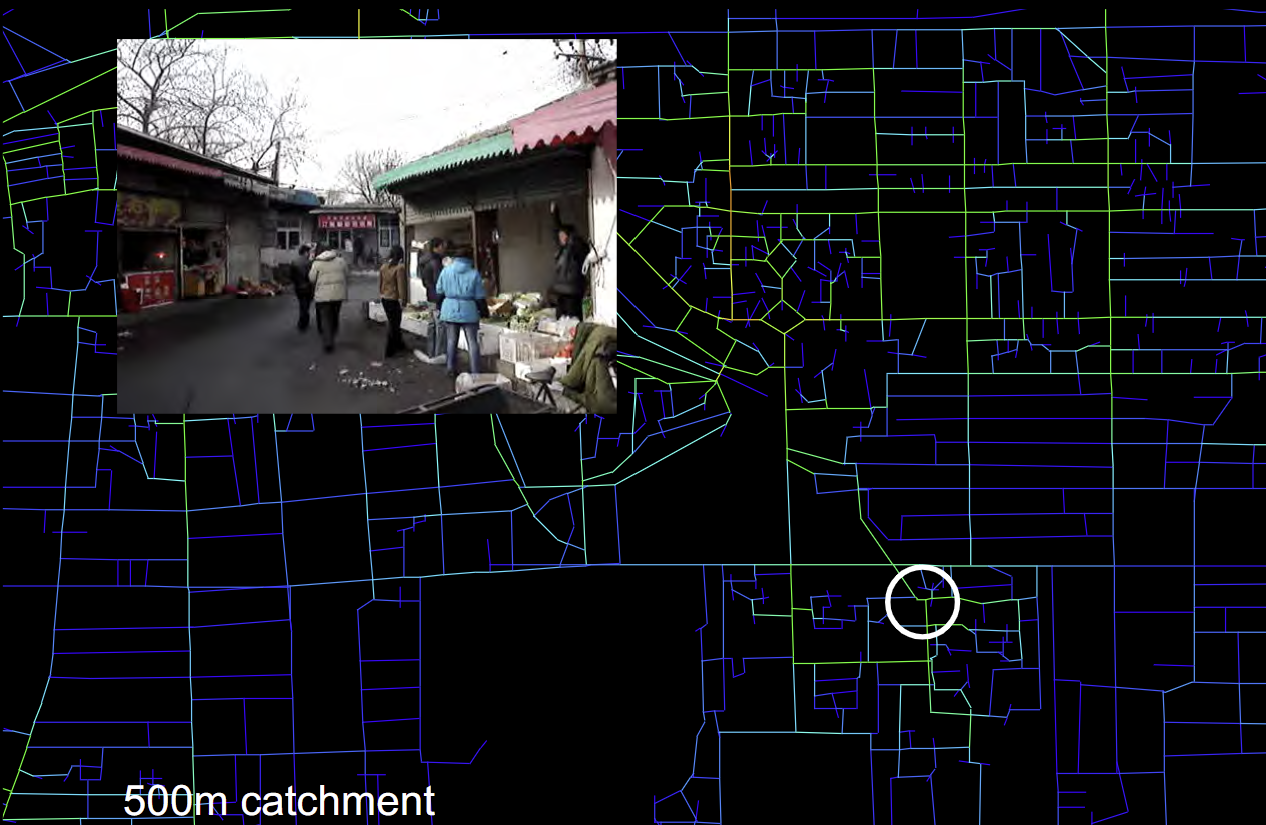
\includegraphics[width=\textwidth]{../assets/ScaleOfObservation1.png}
    \caption{500m Scale}
    \label{fig:ScaleOfObservation1}
  \end{subfigure}
  \begin{subfigure}{0.49\textwidth}
    \centering
    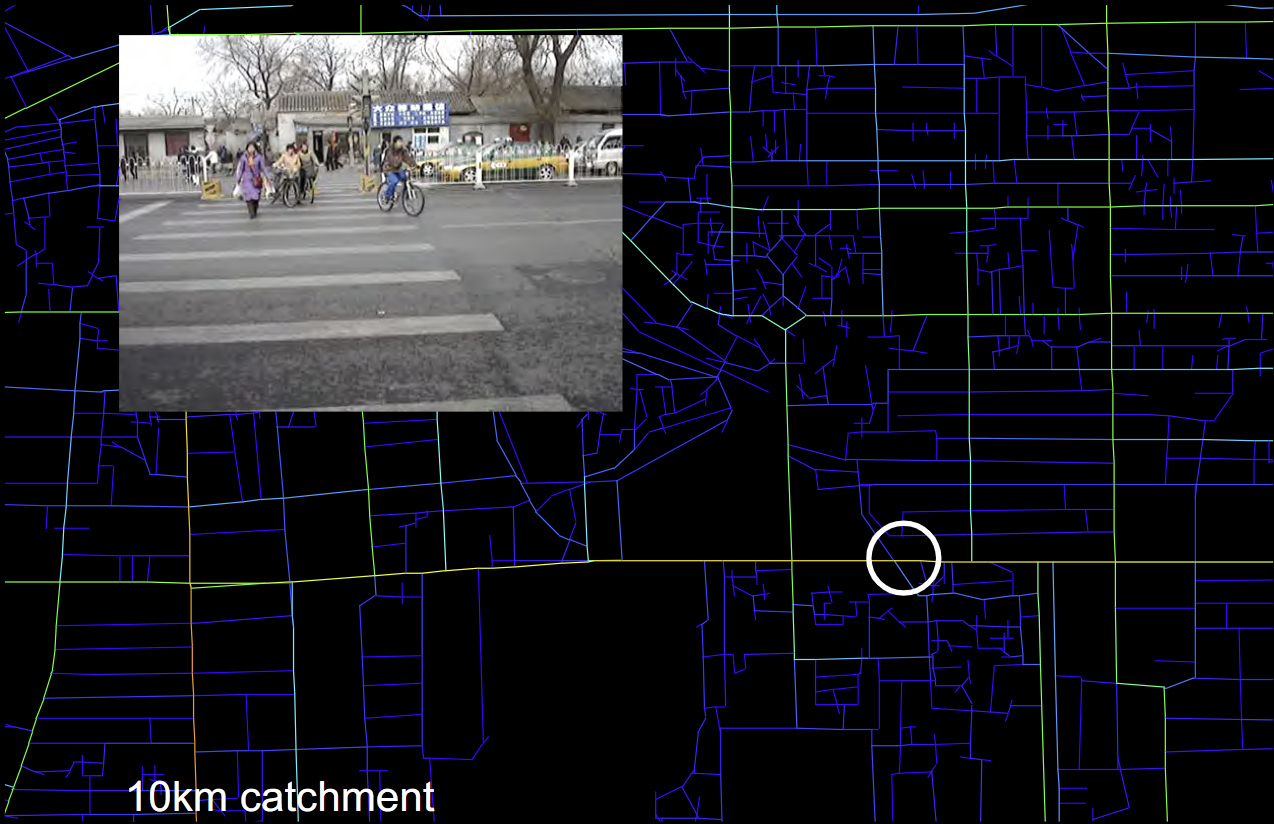
\includegraphics[width=\textwidth]{../assets/ScaleOfObservation2.png}
    \caption{10km Scale}
    \label{fig:ScaleOfObservation2}
  \end{subfigure}
  \caption{Different scale of observation leads to different centre}
\end{figure}

\section{Pedestrian \& Agent Movement}

\subsection{Random Walks}

\subsubsection{Turner \& Penn: A Simplest Experiment}

A simple agent-based simulation (\textbf{\cref{sec:SingleVisualAgent}}), correlates well with observed movement of people, pointing out that there exists a connection between agent movement and axial lines.

\textbf{Aimless} and \textbf{memory-less} agents.

\subsubsection{Turner (2007): Minimal Angle Routes}

Use angular choice to imply route optimisation: Agents will tend to have more probabilities going forward, and more likely to turn small angle other than big ones.

\subsection{Exosomatic}

Exosomatic are the objects in the space, visually guide people navigate in space, e.g. GPS, bridges, escalators, traffic signals, business districts, etc..

Exosomatic will affect agent navigation in following ways:

\begin{itemize}
  \item \textbf{Guidance \& Navigation}: GPS and maps will guide people to the destination via unconventional routes
  \item \textbf{Accessibility}: Bridges, escalators, transport systems changes the accessibility of the space
  \item \textbf{Regulation}: Signals and regulations controls the movement of people
  \item \textbf{Social Influence}: Special zones like business districts, tourist hotspots will attract people beyond the axial connections.
\end{itemize}

\subsubsection{Exosomatic Visual Agent}

Exosomatic visual agent is a random walk agent with vision.

\begin{enumerate}
  \item Each agent will have a vision angle
  \item Agent will pick move direction randomly, but weighted based on the sight length of each direction
  \item After pick a direction, agent will move a fixed distance in that direction and align itself to that direction
  \item Repeat step 2 and 3
\end{enumerate}

Exosomatic visual agent is memoryless and goalless, and because it is a random walk agent, it is also Markovian.

But when looking its movement result, we can find it is similar to the movement from real people. This implies:

\begin{itemize}
  \item Human movement is greatly depend on vision
  \item Navigation can be memoryless but structured
  \item The space structure itself will greatly guide \slash design human movement
  \item Space Syntax metrics aligns with human movement
\end{itemize}

It also explains why axial analysis works. Exosomatic are usually used in smaller scale of space (e.g. crossing, indoor spaces), while axial analysis is usually used in larger scale (e.g. urban level).

\subsection{VGA \& VGA Agent}

\subsubsection{Visual Graph Analysis (VGA)}

VGA is a method for examining the visual relationships within a space. Imagine taking a building or an urban layout, and---at every point in that space---drawing what you can see.

VGA does just that by:

\begin{enumerate}
  \item \textbf{Sampling the Space}:
  \begin{itemize}
    \item A grid of sample points is laid over the area (for example, a museum floor or a city plaza).
  \end{itemize}
  \item \textbf{Calculating Visibility}:
  \begin{itemize} 
    \item At each point, the method computes the ``\textbf{isovist}'' (a polygon representing the area visible from that point).
    \item It then checks which other points in the grid are fully visible from that location.
  \end{itemize}
  \item \textbf{Building the Graph}:
  \begin{itemize}
    \item Each point (node) is connected by edges to every other point it can ``see''.
    \item The connectivity of each node—how many other nodes it can see—is calculated.
  \end{itemize}
  \item \textbf{Deriving Metrics}:
  \begin{itemize}
    \item From the graph, various measures are derived (like overall visibility, connectivity, and integration) that help explain how the space might be experienced or navigated by people.
  \end{itemize}
\end{enumerate}

This process helps quantify how ``open'' or ``enclosed'' different parts of a space are.

\subsubsection{VGA Agent}

VGA Agent is a imaginary pedestrian in the space. Use VGA Agent to \textbf{observe environment and navigate} itself with visual information.

This model moves away from randomness (as in a random walk) and also accounts for the fact that humans react to spatial cues, something exosomatic agents might also influence.

\subsection{Environmental Visual Agent Simulation/System (EVAS)}

EVAS stands for a framework (often interpreted as Environmental Visual Agent Simulation \slash System) that builds on Space Syntax principles---particularly on Visibility Graph Analysis---to simulate how agents (or ``virtual pedestrians'') navigate through spaces.

Essentially, EVAS is a more advanced simulation model that not only considers the static geometric properties of a space (like visibility and connectivity) but also integrates dynamic, environmental cues and human-like decision rules.

EVAS can be thought of as an evolution beyond simple visible-space models. Here's how it functions in simple terms:

\begin{enumerate}
  \item \textbf{Mapping the Environment}:
  \begin{itemize}
    \item Like in Visibility Graph Analysis (VGA), the first step is to sample the space.
    \item A grid (or set of sample points) is laid over the environment, and for each point the visible area (isovist) is calculated.
    \item This produces a detailed map of how parts of the space ``see'' each other.
  \end{itemize}
  \item \textbf{Integrating Additional Cues}:
  \begin{itemize}
    \item EVAS goes beyond pure geometry. It may incorporate additional factors such as:
    \begin{itemize}
      \item Environmental features: Signage, lighting, or obstacles.
      \item Contextual information: Information about where exits, attractions, or congestion points are.
    \end{itemize}
    \item These cues act like exosomatic influences, meaning they are external to the individual but affect navigation decisions.
  \end{itemize}
  \item \textbf{Simulating Agent Behaviour}:
  \begin{itemize}
    \item EVAS agents are virtual pedestrians equipped with decision-making routines.
    \item They ``perceive'' both the visibility information of the space and the extra environmental cues.
    \item Their movement isn't random; they choose paths based on what looks most open, accessible, or strategically useful (similar to human behaviour in unfamiliar or emergency conditions).
  \end{itemize}
  \item \textbf{Dynamic Simulation}:
  \begin{itemize}
    \item The system runs over successive time steps.
    \item As EVAS agents move, the simulation captures how paths are chosen, how traffic might concentrate, and even how evacuation could progress in emergency scenarios.
    \item The dynamic aspect means it can adapt to changes—if an obstacle appears or if a crowd builds up, the agents' decisions can change accordingly.
  \end{itemize}
\end{enumerate}

\chapter{Neural Networks}

\section{Introduction to Neural Networks}

\paragraph{Scale}

Computers (e.g. a CPU) run in high speed (e.g. 2--5GHz) with fewer number of transistors. Brain run at 15--60Hz but with 10\textsuperscript{11} neurons, thus make it able to achieve complex tasks that computers can hardly do.

\paragraph{Massive Parallelism}

A laptop's CPU might have 8--16 processors, but it is far away to the number of neurons in the brain. What's more, the laptop circuits cannot operate in parallel.

However, some structure of the brain can be simulated.

\subsection{Vision and Nurons}

\subsubsection{Exaple: Seeing And Distinguish Number}

For example, a grid of squares shows a pattern of number ``3''. Human eye see it and finally think it is the number 3.

\begin{enumerate}
  \item \textbf{Connection}: Neurons are connected with some other neurons
  \item \textbf{Activate}: If a single neuron receives enough signals from other neurons, it will be activated
  \item \textbf{Result}: Finally, the rod in eye link to something that represents ``3''
\end{enumerate}

In this simulation, the neurons do several things:

\begin{itemize}
  \item \textbf{Inhibit Other Neurons}: If it is activated, stop other neurons from being activated
  \item \textbf{Perform Logical Operations}: Define self activation status based some logical rule
  \item \textbf{``Recovery Period''}: A period of time after activation, the neuron cannot be activated again
\end{itemize}

\subsection{Neuron Models \& Neuron Network}

\subsubsection{Simple Neuron: McCulloch-Pitts Model (1940s)}\label{sec:SimpleNeuron}

Just like real neuron, a neuron in this model has several inputs with different weights, and the final output is the sum of the weighted inputs and an extra threshold.
$$y_i = \mathsf{sign} (\sum w_{ij} x_j - b_i)$$

\subsubsection{Simple Neural Network: Hebbian Learning (1940s)}

Human memory is associative, by context, while computer memory is referenced by location.

\paragraph{Fully Connected Network}

Human can:

\begin{itemize}
  \item Recall memories from partial information
  \item Recognise faces
  \item Associate words
\end{itemize}

To start with, we build a neural network to do the same:

\begin{itemize}
  \item An array of artificial neurons
  \item Connect each neuron to all other neurons
\end{itemize}

\paragraph{Weight of Connection}

Then, the key point to make this network work is the weight.

To make the neuron output reliable, each neuron represents a binary variable, which means its value can either be -1 or 1.

To store a single memory, the weights are set to:
$$w_{ij} = \frac{1}{n} x_i x_j$$

So, if 2 neurons have same value, weight will be positive (\textit{positive reinforcement}), otherwise, negative (\textit{negative reinforcement}).

After this, we can see the outcome of a neuron be like this:
$$y_i = \mathsf{sign} (\sum_{j=1:n} \frac{1}{n} x_i x_j y_j)$$

Now, the network shows the ability to memory: if less than half neurons are wrong, the network will return to the correct state (the original pattern).

Then, we can even extend this process to multiple memories, so the network will be able to remember multiple (suppose that is $p$) states:
$$w_{ij} = \frac{1}{n} \frac{1}{p} \sum_{k = 1:p} x_{ki} x_{kj}$$

\subsection{High Dimensional Space}

\subsubsection{Representing Data in High Dimensional Space}\label{sec:RepresentingDataInHighDimensionalSpace}

Recall the coordinate: A 2D point can be coded with 2 numbers, a 3D point with 3 numbers, and so on. This also means 2 1D points can be coded with 1 2D point, 3 1D points with 1 3D point.

Using similar technique, a two-point system in 3-dimensional space can be represented by 6 numbers, and finally into 1 point in 6-dimensional space.

Take even one step further, if we code the colour with RGB, then a two-point system with point colour can be turned into one point in 12-dimensional space.

\textbf{\textit{As long as the total dimension number is same, data can be converted between different dimensional space.}}

\subsubsection{Linear Algebra Knowledge}

\paragraph{Matrix}

for each neuron, it receives multiple inputs with weights. Mathematically, this step can be represented as a matrix multiplication, the matrix contains weights for each connection.

With the multiplication, the input data is converted to a new space, and the output is the result of the matrix multiplication. The number of dimension of the matrix is defined by the number of dimension of previous layer and next layer.

The outputs are then be added with bias, thus finished the basic process of a layer of neurons.

In addition, because each input data can be converted into a point (or vector), all the inputs (e.g. a dataset) can also construct a matrix, by recording these vectors row by row. \label{DataToPoint1} The weight matrix, however, should record weights for each neuron column by column.

\paragraph{Eigenvalue (特征值) \& Eigenvector (特征向量)}

With matrix multiplication, the data was converted to a new eigenspace. The eigenvector was hidden in the matrix, meaning a direction of characteristic, and the eigenvalue means how important it is in this transform.

And then back to mathematical meaning: Eigenvectors are vectors that is stable (unchanged) during matrix transform; Each eigenvector has a corresponding eigenvalue, which means how much it is changed (\textbf{\cref{sec:ImageAsVectors}}). That's why the eigenvalue represents the importance of the eigenvector.

The matrix multiplication is not always means a reduction of dimension, it in fact means a transformation to goal eigenspace.

\paragraph{Projection}

so, for a matrix that represents a point (vector) of data, what happen to a matrix multiplication? In fact, it is a projection to the direction of eigenvector (\textbf{\cref{fig:VectorProjection1}}).

The mathematical expression is be like this:
$$\mathsf{p_{proj}} = \mathsf{p} \cdot \mathsf{\varphi }$$

Here, p is a point, and $\varphi$ is an eigenvector.

\begin{figure}[htbp]
  \centering
  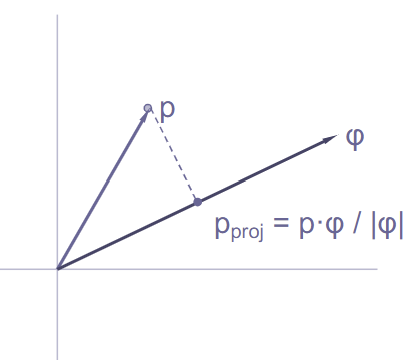
\includegraphics[width=0.3\textwidth]{../assets/VectorProjection1.png}
  \caption{Projection Point to Eigenvector Direction}
  \label{fig:VectorProjection1}
\end{figure}

\chapter{Machine Learning}

\section{Unsupervised Learning}

\subsection{Kohonen Net: Self-Organising Map (SOM)}

Kohonen construct a network based on ``Competitive Learning'', inspired and simulationg the hippocampus of human brain, which is responsible for navigation, thus has a function to represent outside world in 2D.

Now, imagine 2 layer of networks, the first one represents the input, the second one (Kohonen Layer) simulates the hippocampus, the second one is fully connected to the first one.

How does this neural network work? The rule is simple:

\begin{enumerate}
  \item \textbf{Competitive Learning}: The neuron that receives the biggest signal is the winner
  \item \textbf{Strengthening \& Weakening}: The winner neuron will strengthen its connection to the input neurons, and weaken the connection to other neurons.
  \item \textbf{Mapping}: The result is, the Kohonen network will eventually activate the neurons that are similar to the input data.
\end{enumerate}

Because of this mapping phenomenon, Kohonen network is also called ``Self-Organising Map (SOM)''.

There also exist various functions that can be used to calculate strengthening.

\textbf{P.S.} \  In fact, the two layers may not have same dimension, and the Kohonen layer is not necessary to have less dimension or neurons than the input layer.

\subsection{Dynamic Relaxation}\label{sec:DynamicRelaxation}

A method to do form-finding.

Similar to particle system, consider each point as a particle, and each point receives forces from neighbour points based on distance (\textbf{\cref{fig:DynamicRelaxation1}}). Then the equilibrium point position can be calculated as the final position of the point (\textbf{\cref{fig:DynamicRelaxation2}}). Then do this process for all points, and repeat. The outcome will become more and more stable, but alway approximate.

\begin{figure}[htbp]
  \centering
  \begin{subfigure}{0.38\textwidth}
    \centering
    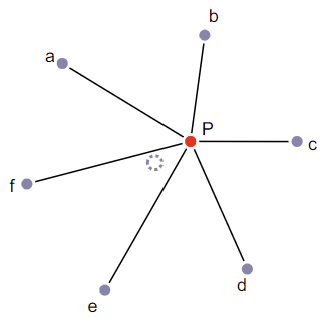
\includegraphics[width=0.5\textwidth]{../assets/DynamicRelaxation1.png}
    \caption{The Particle Relationship in Dynamic Relaxation}
    \label{fig:DynamicRelaxation1}
  \end{subfigure}
  \begin{subfigure}{0.38\textwidth}
    \centering
    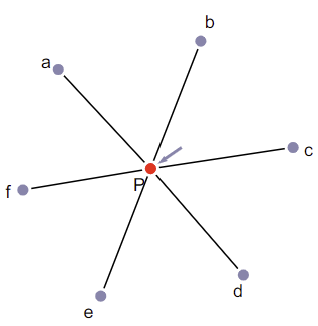
\includegraphics[width=0.5\textwidth]{../assets/DynamicRelaxation2.png}
    \caption{A Simple Version of Dynamic Relaxation}
    \label{fig:DynamicRelaxation2}
  \end{subfigure}
  \caption{Simple Dynamic Relaxation}
\end{figure}

Other kind of forces (e.g. gravity, load, etc.) can be added into the system as well (\textbf{\cref{fig:DynamicRelaxation3}}). And we can also apply weight to each force to control the effect of each force (\textbf{\cref{fig:DynamicRelaxation4}}).

\begin{figure}[htbp]
  \centering
  \begin{subfigure}{0.38\textwidth}
    \centering
    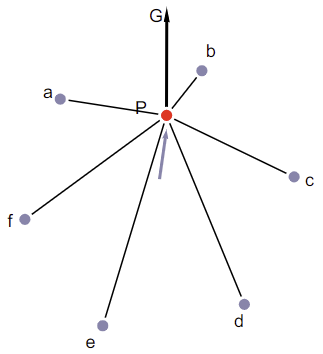
\includegraphics[width=0.5\textwidth]{../assets/DynamicRelaxation3.png}
    \caption{Apply Gravity to System}
    \label{fig:DynamicRelaxation3}
  \end{subfigure}
  \begin{subfigure}{0.38\textwidth}
    \centering
    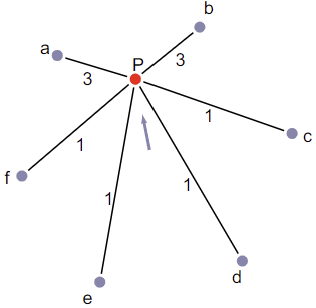
\includegraphics[width=0.5\textwidth]{../assets/DynamicRelaxation4.png}
    \caption{Add Weight to System}
    \label{fig:DynamicRelaxation4}
  \end{subfigure}
  \caption{More Complex Dynamic Relaxation}
\end{figure}

After all, the way to calculate equilibrium point should be this:
$$\mathsf{X}_i = \mathsf{X}_i + \sum_{j} \frac{\mathsf{Tension}_{ij}}{\mathsf{Length}_{ij}} (\mathsf{X}_j - \mathsf{X}_i)$$

\subsubsection{Finite State Method}\label{sec:FiniteStateMethod}

Finite State Method (FEM) is a kind of method that divide an object into a series of small parts (e.g. triangles, particles, etc.), and calculate the forces between them.

Sometimes, Dynamic Relaxation (\textbf{\cref{sec:DynamicRelaxation}}) is used as one of the solutions of FEM, and obviously, FEM uses Euler method (\textbf{\cref{sec:EulerMethod}}) as well.

\subsection{Runge-Kutta Method}\label{sec:RungeKuttaMethod}

\subsubsection{Euler Method}\label{sec:EulerMethod}

The dynamic relaxation in fact is using the Euler method. Euler method is a simple way to find numerical solution by stepping forward with slight movements.

The outcome is always not absolute stable, but as long as the value is changing in a small enough range, we can consider it as stable.

\subsubsection{Midpoint Method}\label{sec:MidpointMethod}

Midpoint method improves Euler method. It calculates the the previous point and next point to estimate slope of the midpoint, and use the midpoint slope to estimate the solution. It is more complex than the Euler method, but it is more accurate (\textbf{\cref{fig:RungeKutta1}}).

\begin{figure}[htbp]
  \centering
  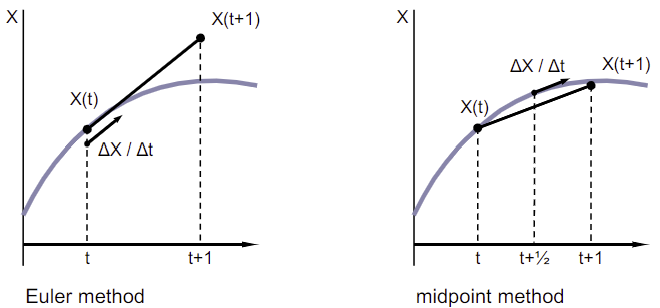
\includegraphics[width=0.5\textwidth]{../assets/Runge-Kutta1.png}
  \caption{Comparison between Euler Method and Midpoint Method}
  \label{fig:RungeKutta1}
\end{figure}

\subsubsection{Runge-Kutta Methods}

In fact, Euler method and Midpoint method are all special cases of Runge-Kutta methods. Runge-Kutta methods may use multiple points to estimate the slope that would be used to calculate the solution.

The most common Runge-Kutta method is \textit{fourth-order Runge-Kutta}. It uses the previous point slope, 2 midpoint slopes to calculate the fourth slope, and use these four slopes to calculate the solution.

\section{Supervised Learning}

Supervised learning means the network learns what it is told. It was trained with a dataset (the input and the true output).

\subsection{Perceptron: Supervised Pattern Classifier}

Perceptron was first proposed by Rosenblatt in 1960s, based on a model of visual perceptron.

$$\mathsf{Image} \xrightarrow[]{\textsf{encoding}} \mathsf{Perceptron Input} \xrightarrow[]{\textsf{classification}} \textsf{Perceptron Output}$$

Recall how do a neuron get its result (\textbf{\cref{sec:SimpleNeuron}}):

$$y = \mathsf{sign} (\sum w_i x_i + b)$$

If we do a simplification, we can consider the bias also as an weight, with a fixed input:
$$y = \mathsf{sign} (\textit{w} \cdot \textit{x}) \qquad \mathsf{or} \qquad y = \mathsf{sign} (w \cdot x + w_0)$$

\subsubsection{Classification}

Now let us consider the data in dataset. As previous mentioned, these data can be represented as a series of points (\textbf{\cref{sec:RepresentingDataInHighDimensionalSpace}}) (and even record them as one matrix (\textbf{\cref{DataToPoint1}})). On the other hand, the output equation, means a vector equation of a line in that space (e.g. plane, hyperplane, etc.).

In this expression, $w$ is the normal vector of this line, and the $w_0$ bias vector will move this line on all axis. More exactly, you can project the bias vector to the normal vector, and the distance $\frac{w_0}{\lVert z \rVert}$ is exact how far the line is moved (\textbf{\cref{fig:PerceptronClassification1}}).

\begin{figure}[htbp]
  \centering
  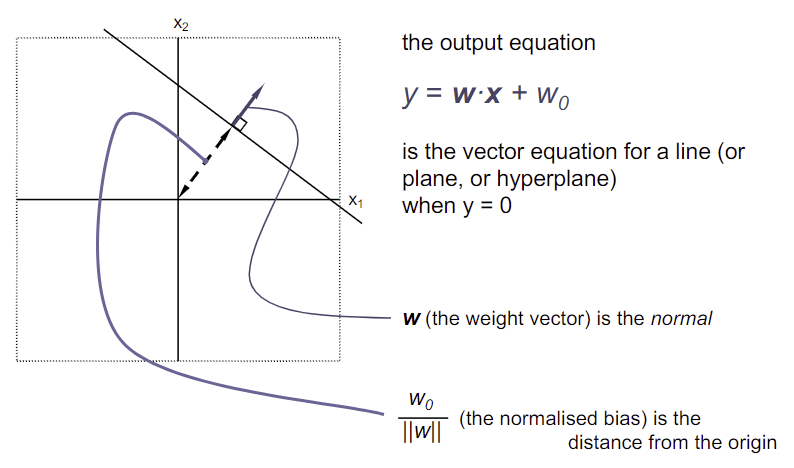
\includegraphics[width=0.5\textwidth]{../assets/Perceptron1.png}
  \caption{Neural Network draw a line in high dimensional space}
  \label{fig:PerceptronClassification1}
\end{figure}

And now, we can control the line to do the classification (\textbf{\cref{fig:PerceptronClassification2}}).

\begin{figure}[htbp]
  \centering
  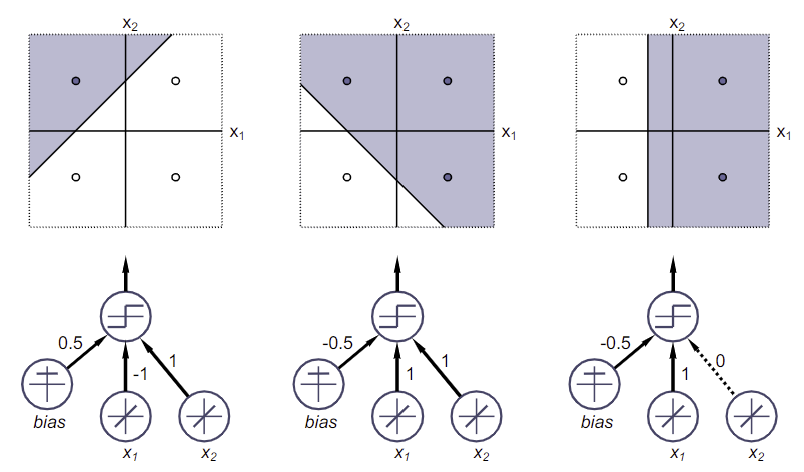
\includegraphics[width=0.5\textwidth]{../assets/Perceptron2.png}
  \caption{Control the line to do the classification}
  \label{fig:PerceptronClassification2}
\end{figure}

\subsubsection{Adjusting Weights}

Now go to more practical part, how to adjust the line so we can adjust the boundary.

The output of the misclassified neurons determines the size of error \textbf{J} ($\mathsf{J} = \lVert w \cdot x \rVert$).

Now, we can transform the normal vector of the line (by add a vector $\mathsf{J}x$) to adjust the boundary (\textbf{\cref{fig:AdjustWeight1}}), which means in fact we are adjusting the weights. But in fact it is a gradual adjustment controlled by the \textit{learning rate} $\eta$, so finally, for each unclassified point, update:
$$w = w + \eta J x$$

\begin{figure}[htbp]
  \centering
  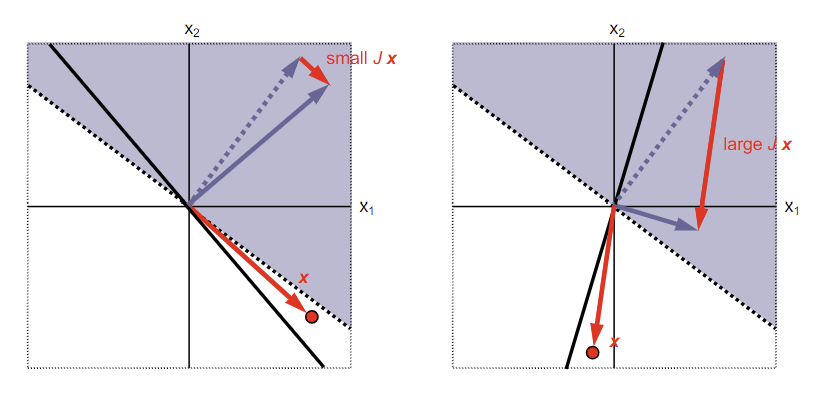
\includegraphics[width=0.5\textwidth]{../assets/AdjustWeight1.png}
  \caption{Adjust the normal vector to adjust the boundary}
  \label{fig:AdjustWeight1}
\end{figure}

\subsubsection{Acticateion Function}

Up till now, we use the sign function as the activation function, so we can get only binary output (1 or -1). In fact, there are many other activation functions, we use them depend on the need (what kind of out put we want, how sensitive the output is to the input, etc.).

One of the typical active function is the \textit{sigmoid function} (\textbf{\cref{fig:SigmoidFunction}}):
$$y = \frac{1}{1 + e^{-w \cdot x}}$$

\subsection{XOR Problem}

Let's go one step further! There are some classification mission that one single line cannot solve, for example, XOR problem (\textbf{\cref{fig:XOR}}).

\begin{figure}[htbp]
  \centering
  \begin{subfigure}{0.3\textwidth}
    \centering
    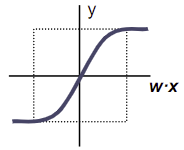
\includegraphics[width=0.8\textwidth]{../assets/ActivationFunction1.png}
    \caption{Sigmoid function}
    \label{fig:SigmoidFunction}
  \end{subfigure}
  \begin{subfigure}{0.3\textwidth}
    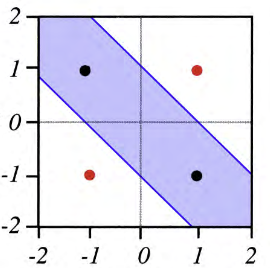
\includegraphics[width=0.6\textwidth]{../assets/XOR1.png}
    \caption{A typical graph showing a XOR problem}
    \label{fig:XOR}
  \end{subfigure}
\end{figure}

\subsubsection{Multi-Layer Perceptron (MLP)}\label{sec:MLP}

One layer perceptron can divide the space into two parts and choose one of them (\textbf{\cref{fig:MLP1}}), so one way to solve XOR problem is to this process multiple times so we can get a specific part of the sapce (\textbf{\cref{fig:MLP2}}). This kind of solution is called \textbf{Multi-Layer Perceptron} (MLP).

\begin{figure}[htbp]
  \centering
  \begin{subfigure}{0.49\textwidth}
    \centering
    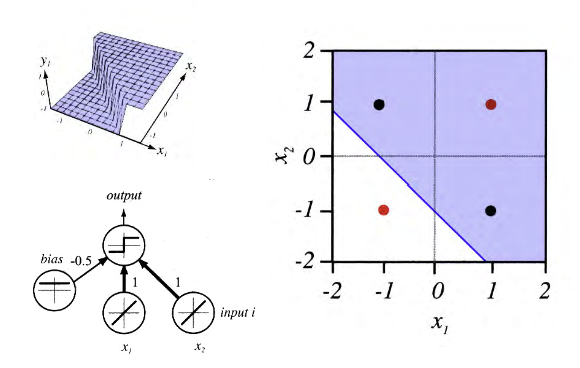
\includegraphics[width=\textwidth]{../assets/MLP1.png}
    \caption{Linear equation pick half of the space}
    \label{fig:MLP1}
  \end{subfigure}
  \begin{subfigure}{0.49\textwidth}
    \centering
    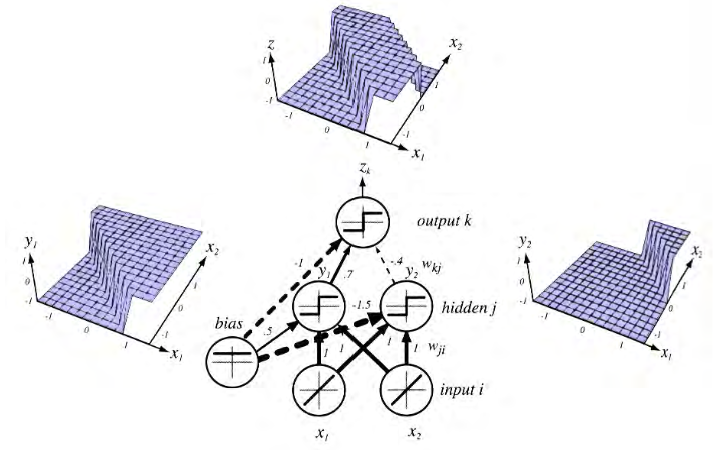
\includegraphics[width=\textwidth]{../assets/MLP2.png}
    \caption{Two layers of perceptron can pick a middle part of the space}
    \label{fig:MLP2}
  \end{subfigure}
\end{figure}

\subsubsection{Support Vector Machine (SVM)}\label{sec:SVM}

Another solution is called \textbf{Support Vector Machine} (SVM). It use an interesting idea to solve this problem: find a higher dimensional line to do the classification.

More interestingly, it can automatically find the optimal division, which will make two class of data far away from each other (\textbf{\cref{fig:SVM1}}).

\begin{figure}[htbp]
  \centering
  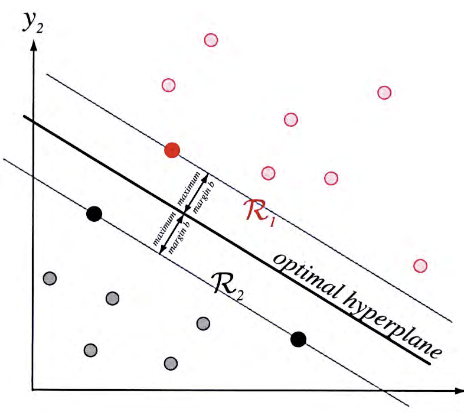
\includegraphics[width=0.3\textwidth]{../assets/SVM1.png}
  \caption{SVM will find the optimal hyperplane to do the classification}
  \label{fig:SVM1}
\end{figure}

\section{Two Type of Learning: Classification \& Regression}

Now, we have understood the basic of Artificial Neural Network (ANN), which can do more than traditional linear regression method.

\paragraph{Classification}

Classification is to deal with data that need to be classified into different classes, and the learning is used to find the boundary between these sets.

We can even find the non-linear boundary in high dimensional space with MLP (\textbf{\cref{sec:MLP}}) and SVM (\textbf{\cref{sec:SVM}}).

\paragraph{Regression}

In the regression problem, all data is in the same class, the learning is used to find the function that best fits these points.

Comparing with linear regression, ANN can deal with non-linear regression function.

\section{Practical Uses}

\subsection{Structure Design: Apply SVM to An Optimisation Algorithm}

A simple method: place modular units arrayed throughout the volume, thus can construct a structure.

\subsubsection{Dataset: Use Gradient Descent \slash Ascent}

Use gradient descent \slash ascent to do optimisation:

\begin{itemize}
  \item Move in the direction that increases /slash decreases the fitness
  \item Can apply to anything as long as it has a \textit{quantifiable fitness function}
\end{itemize}

\subsubsection{Calculate Fitness with FEM}

Finite Element Method (FEM) (\textbf{\cref{sec:FiniteStateMethod}}) breaks solid object into many simple members for analysis. This method is widely used to simulate stress and deformation when forces are applied to given object.

In this method, the space frame already consists of simple members.

Each applied force has an ideal structure.

\paragraph{Machine Learning to Get Optimal Node Position}

In traditional workflow, we need GA and FEM to get the optimal structure. But a neural network can take place of them.

\subsubsection{Machine Learning to Get Optimal Node Position}

In traditional workflow, we need GA and FEM to get the optimal structure. But a neural network can take place of them.

\begin{itemize}
  \item \textbf{Input}: The applied force
  \begin{itemize}
    \item \textbf{Number}: Number of coordinate axis (e.g. 2 for 2D forces, 3 for 3D forces)
  \end{itemize}
  \item \textbf{Output}: The optimal node positions
  \begin{itemize}
    \item \textbf{Number}: Number of coordinates of nodes. (e.g. if there are 4 nodes in 3D, then that's $4 \times 3 = 12$)
  \end{itemize}
\end{itemize}

In this process, suppose the dataset \textbf{D} has input vector \textbf{x} and response vector \textbf{y}, then it contains a function to be learned:
$$\mathsf{y} = f(\mathbf{x})$$

The SVM will learn from the dataset to approximate the function by building a model $f'(\mathbf{x})$, thus the SVM is able to estimate the best output.

\subsubsection{Potential Problem of Gradient Descent \slash Ascent}

This kind of method will face one serious issue: \textbf{local optima}. This means there exists a hill or valley in the fitness function, but is not the biggest one, but gradient method will stuck in this kind of optima, thus cannot find the global optima.

\subsubsection{Overfitting}

The data or raw data in dataset not converged in a line, which means there exists noise that is not helpful. Overfitting means the model also learn the noise, which will make the model not generalised.

\subsubsection{Conclusion}

\begin{itemize}
  \item GD can solve the structural shape optimization problem, but only within an acceptable variance in node positions
  \item Variance causes some of the optimized geometries in the training set to fall slightly below the true optimal solution (like noise)
  \item Regression process performed by the SVM effectively ``smoothes out'' the function
\end{itemize}

By using the learned, continuous function to derive the structural geometry, the transitions between adjacent cubes are smoother, and the composite structure benefits in strength.

\section{Machine Perception \& Vision}

\subsection{Image Processing}

\paragraph{Representation of Image}\label{sec:ImageRepresentation}

Image is constructed by pixels, and each pixel can be represented by a greyscale number or RGB value, thus an image can be represented by a series of numbers.

\subsubsection{Image Noise}

Noise is random or systematic disturbance in image, resulting blur, noise points and other problems. These useless extra information will affect performance of Neural Network.

\paragraph{Gaussian Noise}

\begin{figure}[htbp]
  \centering
  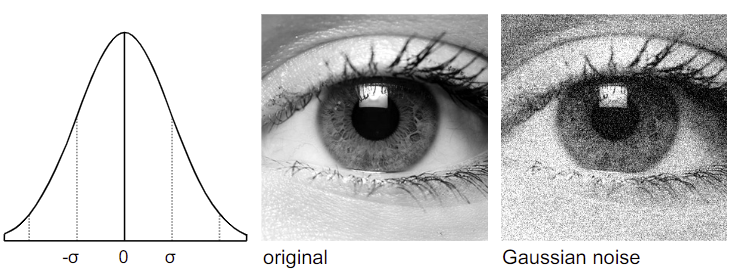
\includegraphics[width=0.6\textwidth]{../assets/GaussianNoise1.png}
  \caption{Gaussian Distribution and Gaussian Noise}
  \label{fig:GaussianNoise1}
\end{figure}

Gaussian noise is one of the most common types of noise, showing slight brightness or colour change on image. It is random and can be represented by a Gaussian distribution (\textbf{\cref{fig:GaussianNoise1}}).
$$p(x) = \frac{1}{\sqrt{2 \pi \sigma^2}} \exp (-\frac{(x - \mu)^2}{2 \sigma^2})$$

\paragraph{Smooth Image with Linear Filter}

\subparagraph{Linear Filter}

One way to smoothen image by pick neighbouring pixels and average them to determine the central pixel. This method is called linear filter.
$$I_A(i, j) = I \times A = \sum_{h=-\frac{m}{2}}^{\frac{m}{2}} \sum_{k=-\frac{m}{2}}^{\frac{m}{2}} A(h, k) I(i + h, j + k)$$

By applying the linear filter, the image will be like below:

\begin{figure}[htbp]
  \centering
  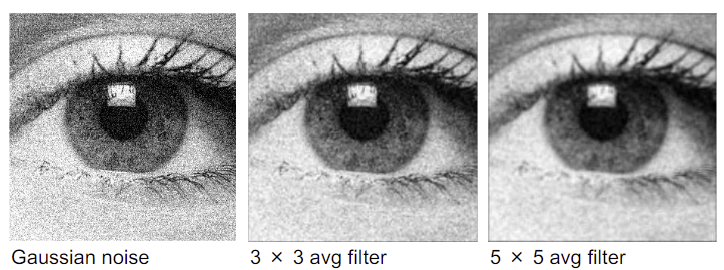
\includegraphics[width=0.6\textwidth]{../assets/LinearFilter1.png}
  \caption{Linear Filter}
\end{figure}

\subparagraph{Gaussian Filter}

Gaussian distribution can also applied as a filter. This filter will make the image more smooth, but the image will be blurred, thus it is also called ``Gaussian blur'' (\textbf{\cref{fig:GaussianFilter1}}).

\begin{figure}[htbp]
  \centering
  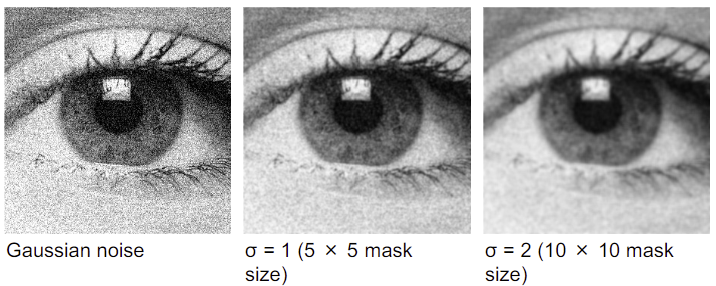
\includegraphics[width=0.6\textwidth]{../assets/GaussianFilter1.png}
  \caption{Gaussian Filter}
  \label{fig:GaussianFilter1}
\end{figure}

Range -2σ to 2σ subtends about 89.75\% of the total area (typically use a mask width of 5σ).

A 2d Gaussian is Gaussians in each dimension (we can separate them in practice).

\subsubsection{Edge Detection}

\paragraph{Roberts Edge Detector}

The very first edge detector, use a \textit{kernel} (a rectangular filter) to detect brightness change, and then calculate the feature magnitude.

\subparagraph{Find Local Features with Filters}

2 filters are used to detect edges from left top to right bottom and from right top to left bottom.

$$G_x = \begin{bmatrix} +1 & 0 \\ 0 & -1 \end{bmatrix} \quad G_y = \begin{bmatrix} 0 & +1 \\ -1 & 0 \end{bmatrix}$$

\subparagraph{Calculate Feature Magnitude}

$$G = \sqrt{G_x^2 + G_y^2}$$

\subparagraph{Mark Pixels with Threshold}

\begin{figure}[htbp]
  \centering
  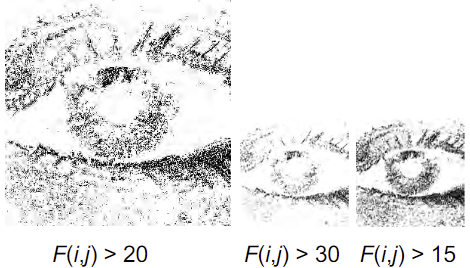
\includegraphics[width=0.45\textwidth]{../assets/RobertsEdgeDetector1.png}
  \caption{Roberts Edge Detector}
\end{figure}

\paragraph{Sobel Edge Detector}

Sobel edge detector is a stronger one, running with a 3x3 convolutional kernel.

\subparagraph{Find Local Gradients with Filters}

Here uses 2 filters to detect edge, one horizontal and one vertical.

The horizontal one:
$$G_x = \begin{bmatrix} -1 & 0 & +1 \\ -2 & 0 & +2 \\ -1 & 0 & +1 \end{bmatrix}$$

The vertical one:
$$G_y = \begin{bmatrix} -1 & -2 & -1 \\ 0 & 0 & 0 \\ +1 & +2 & +1 \end{bmatrix}$$

\subparagraph{Calculate Feature Magnitude}

$$G = \sqrt{G_x^2 + G_y^2}$$

\subparagraph{Mark Pixels with Threshold}

\begin{figure}[htbp]
  \centering
  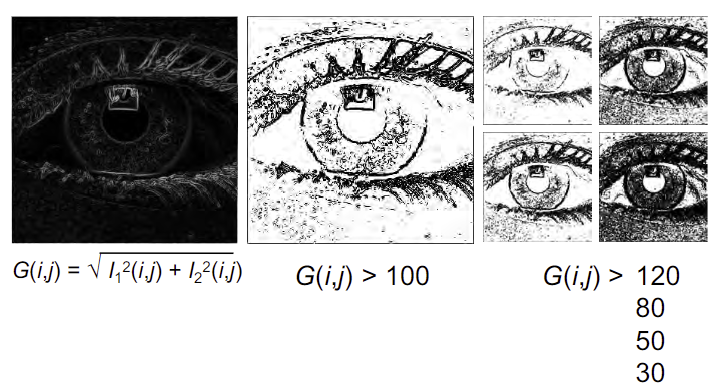
\includegraphics[width=0.45\textwidth]{../assets/SobelEdgeDetector1.png}
  \caption{Sobel Edge Detector}
\end{figure}

\paragraph{Canny Edge Detector}

This is the most powerful one.

\subparagraph{Filter Noise}

A Gaussian Filter is applied to blur the image and remove noise.
$$G = \frac{1}{16} \begin{bmatrix} 1 & 2 & 1 \\ 2 & 4 & 2 \\ 1 & 2 & 1 \end{bmatrix}$$

\subparagraph{Calculate Gradients}

Use Sobel filter to calculate gradients.

Then compute the edge strength:
$$E_S(i, j) = \sqrt{{J_x}^2 (i, j) + {J_y}^2 (i, j)}$$

And edge orientation:
$$E_O(i, j) = \arctan \frac{J_y (i, j)}{J_x (i, j)}$$

\begin{figure}
  \centering
  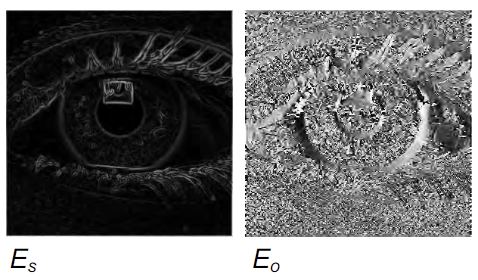
\includegraphics[width=0.3\textwidth]{../assets/CannyEdgeDetector1.png}
  \caption{Image of $E_S$ and $E_O$}
\end{figure}

\subparagraph{Thresholding}

\begin{figure}
  \centering
  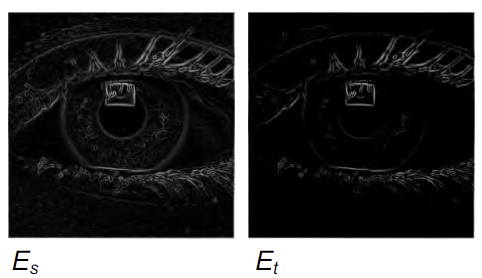
\includegraphics[width=0.3\textwidth]{../assets/CannyEdgeDetector2.png}
\end{figure}

\subparagraph{Non-Max Suppression}

The wanted edges are centres of edges (1 pixel wide).

For each find $E_O(i, j)$, find the closest direction $d_k$, compare $E_S(i, j)$ against its neighbours in direction $d_k$ (\textbf{\cref{fig:CannyEdgeDetector3}}).

\begin{figure}
  \centering
  \begin{subfigure}{0.4\textwidth}
    \centering
    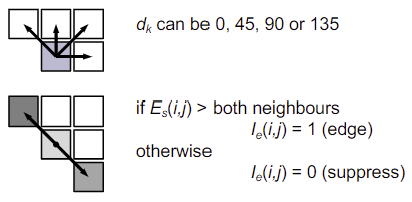
\includegraphics[width=\textwidth]{../assets/CannyEdgeDetector3.png}
    \caption{Non-Max Suppression}
    \label{fig:CannyEdgeDetector3}
  \end{subfigure}
  \begin{subfigure}{0.4\textwidth}
    \centering
    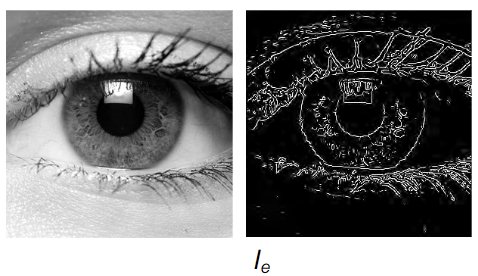
\includegraphics[width=\textwidth]{../assets/CannyEdgeDetector4.png}
    \caption{Final Outcome of Canny}
  \end{subfigure}
\end{figure}

\subsubsection{Image As Vectors}\label{sec:ImageAsVectors}

As previously mentioned, data (\textbf{\cref{sec:RepresentingDataInHighDimensionalSpace}}) including image (\textbf{\cref{sec:ImageRepresentation}}) can be represented by a vector or point in high dimensional space. Furthermore, batch of data can also constructed as a matrix (\textbf{\cref{DataToPoint1}}).

So, what does \textbf{eigenvector} and \textbf{eigenvalue} mean in this context?

\paragraph{Example: ``Eigenfaces'' in Convolutional Neural Network}

Here, we take face recognition as an example. 26 different faces as a dataset was converted into points in 900 dimensional space (\textbf{\cref{fig:Eigenfaces1}}).

\begin{figure}[htbp]
  \centering
  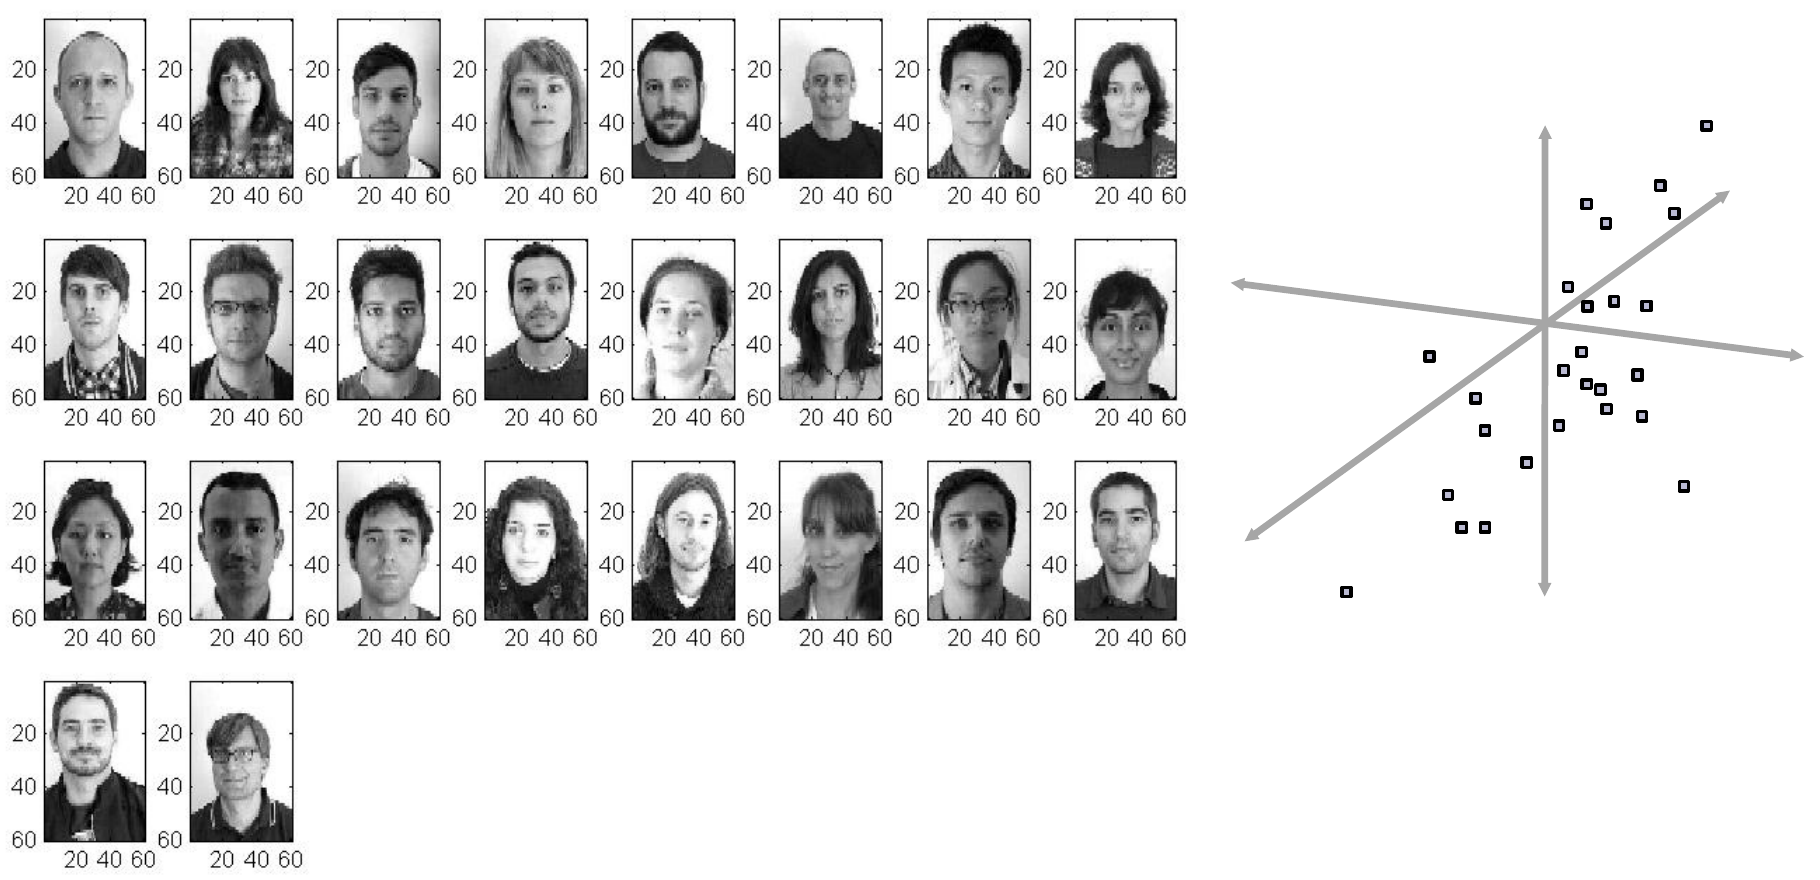
\includegraphics[width=0.7\textwidth]{../assets/Eigenfaces1.png}
  \caption{26 faces and corresponding points in space}
  \label{fig:Eigenfaces1}
\end{figure}

\subparagraph{Measure Difference between Faces}
If we find the eigenvectors, we can project these points on those vectors.

Now these faces can be represented as a linear combination of the eigenvectors (\textbf{\cref{fig:Eigenfaces2}}).

\begin{figure}[htbp]
  \centering
  \begin{subfigure}{0.3\textwidth}
    \centering
    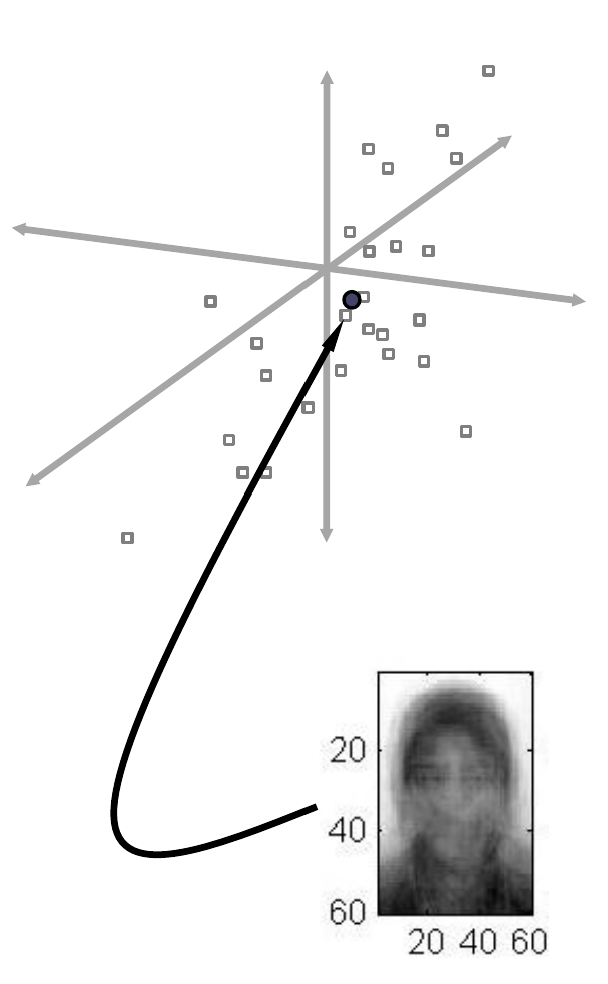
\includegraphics[width=0.5\textwidth]{../assets/MeanPointFace1.png}
    \caption{Face of the mean point (``Eigenface'')}
  \end{subfigure}
  \begin{subfigure}{0.66\textwidth}
    \centering
    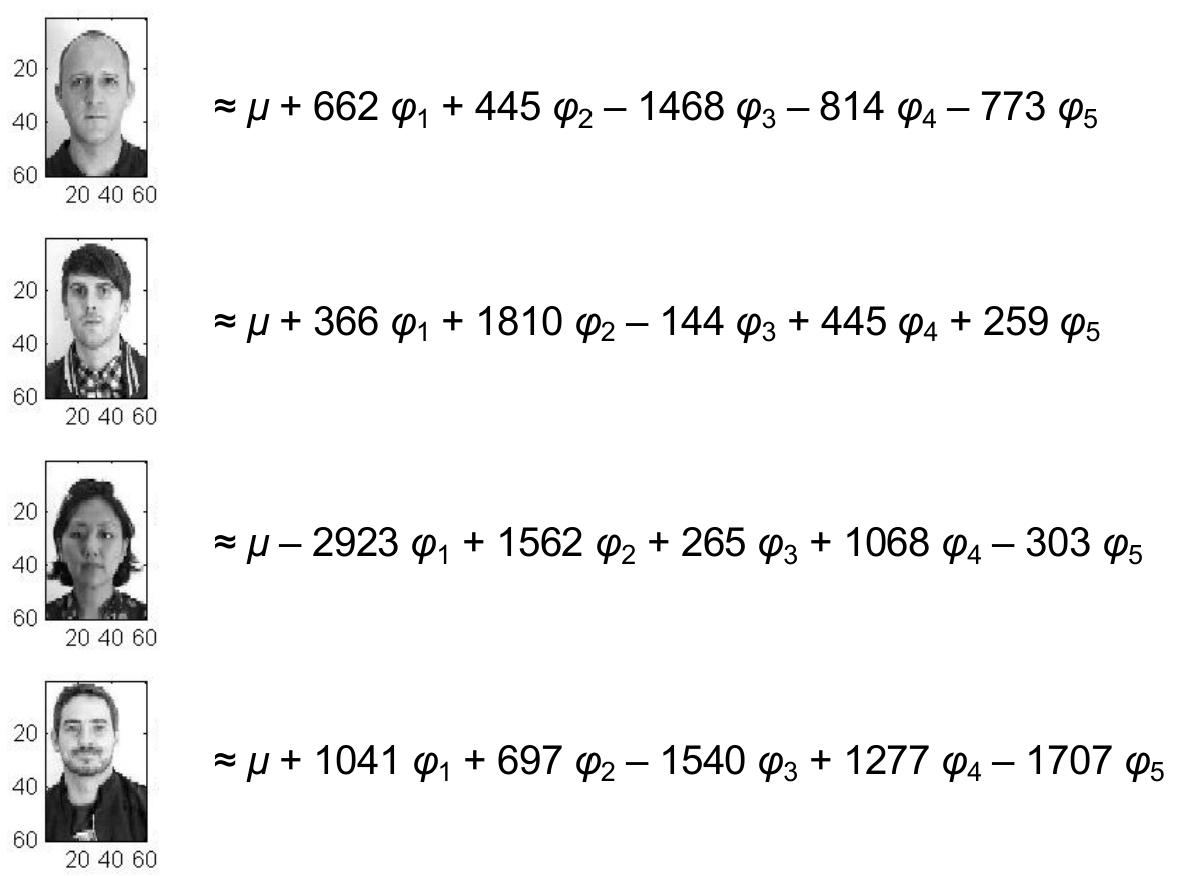
\includegraphics[width=0.6\textwidth]{../assets/Eigenfaces2.png}
    \caption{Represent faces with eigenvectors}
    \label{fig:Eigenfaces2}
  \end{subfigure}
\end{figure}

In this way, we can measure the difference between faces.

The 26 face dataset has 25 dimensions of variances.

\subparagraph{Reconstruction}

Similarly, more faces we have in dataset, the better quality we will get in generating a new image(\textbf{\cref{fig:Eigenfaces3}}).

\begin{figure}[htbp]
  \centering
  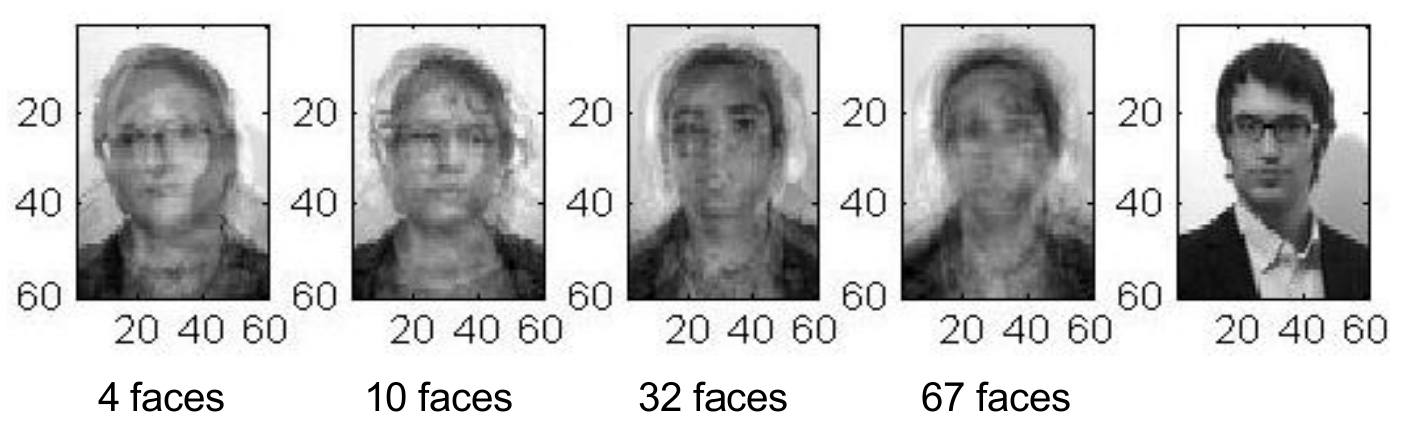
\includegraphics[width=0.8\textwidth]{../assets/Eigenfaces3.png}
  \caption{Reconstruction of face}
  \label{fig:Eigenfaces3}
\end{figure}

\chapter{Emergence 涌现 \& Convergence 收敛}

\section{Complex System \& Generative Design}

There are several methods to do such design:
\begin{itemize}
  \item Grammar
  \item Cellular Automata
  \item Stochastic Iteration 随机迭代
\end{itemize}

Complex from simple rules: \textbf{Emergence}

Same from different rules: \textbf{Convergence}

\begin{enumerate}
  \item Generating a shape
  \item emergence:
  \begin{itemize}
    \item history drawing and design
    \item a generative project \textit{exposure} (\cref{fig:Exposure1})
  \end{itemize}
  \item convergence:
  \begin{itemize}
    \item building simulations and models
    \item projects incorporating analysis, structural optimisation
  \end{itemize}
\end{enumerate}

\section{Emergence}

\textbf{Emergence} is a property of a complex system, in which the behaviour of the whole system cannot be predicted by the behaviour of the parts taken separately.

\begin{itemize}
  \item Grammar
  \begin{itemize}
    \item L-system
    \item Fractal 分形
  \end{itemize}
  \item Cellular Automata
  \item Stochastic Iteration
\end{itemize}

\subsection{Development of Engineering}

\subsubsection{10,000 BC -- 1500 AD: Technology of Analysis}

\begin{itemize}
  \item Enlightenment tools provided the ability to view the great breadth of a project from a single point.
  \item Tendency toward reductionism: make complex problems manageable
  \item Traditional engineering: strict hierarchy 层次结构
  \begin{itemize}
    \item Primary members support secondary support tertiary, etc.
    \item Total energy consumed by the system accumulates at each step
  \end{itemize}
\end{itemize}

\subsubsection{1960s: Technology of Simulation}

\begin{itemize}
  \item Form finding: 1960s
  \item ``Physical model is a necessity''
  \item Cannot calculate
\end{itemize}

\subsubsection{Middle 20\textsuperscript{th} Century: Complexity}

John Argyris pushed out \textit{Finite Element Method}: breaks solid object into many simple members for analysis.

Buckminster Fuller: ``Synergy means behaviour of whole systems
unpredicted by the behaviour of their parts taken separately''

\begin{itemize}
  \item Individual components act together, usually to greater benefits
  \item Designing the rules, not the final product.
\end{itemize}

\paragraph{Warren Weaver: three stages in the history of scientific thought}

\begin{enumerate}
  \item Problems of Simplicity
  \item Problems of Disorganised Complexity
  \item Problems of Organised Complexity
\end{enumerate}

\subsection{Generative Design}

\begin{itemize}
  \item Design activity is focused on the set of rules, or the \textit{process}
  \item The final product is \textit{emergent}
\end{itemize}

\subsubsection{Antony Gormley's \textit{Exposure} (\textbf{\cref{fig:Exposure1}})}

\paragraph{Method 1: Cellular Automata Models}

\subparagraph{Find Points of Greatest Curvature: Phyllotaxis 叶序}

In each step:
\begin{enumerate}
  \item Incerment cell\textsubscript{value}
  \item cell\textsubscript{value} = cell\textsubscript{value} - cell\textsubscript{deplete}
  \item cell\textsubscript{value} > threshold $\rightarrow$
  \begin{enumerate}
    \item bud
    \item cell\textsubscript{deplete} = 1
  \end{enumerate}
  \item neighbour cell\textsubscript{deplete} > 0 $\rightarrow$ cell\textsubscript{deplete} = neighbour cell\textsubscript{deplete}
\end{enumerate}

Then, run cellular automata on the shape (irregular mesh), use phyllotaxis algorithm to get the conflict nodes.

\subparagraph{Connect Nodes: Voronoi Tessellation 沃罗诺伊镶嵌}

Vertices at the intersection of three cells

Use Voronoi tessellation to connect nodes and convert points into polygons.

\paragraph{Method 2: Grammars}

\subparagraph{Branching: Member growth within the surface}

\subsubsection{Method 3: Stochastic Iteration}

\subparagraph{Interior Points: Adjustment and Smoothing}

\subparagraph{Dynamic Relaxation (\textbf{\cref{sec:DynamicRelaxation}})}

\subsection{Strict Definition of Emergence}

The computation is incompressible: there is no faster computation to generate the output of the system than the system itself

\subsubsection{Elegance}

A program is ``elegant'' if no smaller program has the same output. (Gregory Chaitin)

\subsubsection{Kolmogorov Complexity}

The length of the string's shortest description in some universal (programming) language. (Andrey Kolmogorov et al.)

We cannot know whether a string is complex: 

Chaitin's incompleteness theorem says this can't be proved for a specific string (similar to Gödel's theorem).

There may always be a more compressed way of computing
the output.

Simulation of vast, complex systems is possible.

\section{Convergence}

Similar behaviour from disparate parts, also \textbf{the reason we are able to do simulation \slash analysis}.

\subsection{State Space}

State space is to describe a system as a vector field:

\begin{itemize}
  \item One axis for each system variable
  \item Each state is a point
  \item Each has a vector directing to the next state
  \item fully deterministic
\end{itemize}

\subsubsection{Divergent}

\begin{itemize}
  \item Complex behaviour from simple rules
  \item Small initial change leads to big effect
\end{itemize}

\subsubsection{Convergent}

\begin{itemize}
  \item ``Basin of attraction'' in state space
  \item All start conditions go to the same end
\end{itemize}

\subsection{Example: Individual Moving Agents}

\subsubsection{Two Groups of Particles Crushing Together}

\begin{figure}[htbp]
  \centering
  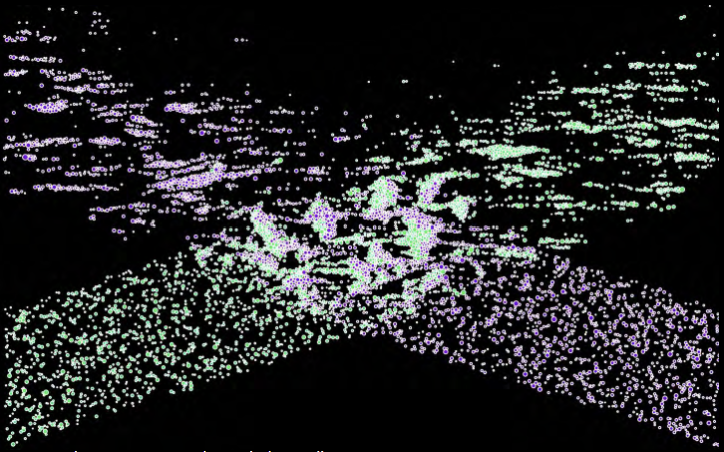
\includegraphics[width=0.4\textwidth]{../assets/GroupParticles1.png}
\end{figure}

\subsubsection{Single Visual Agent}\label{sec:SingleVisualAgent}

Rule for single agent:

\begin{itemize}
  \item Choose any location you can see (within 170$\circ$ field of view)
  \item Move 3 steps towards it
  \item Choose another location
\end{itemize}

And the result be like below:

\begin{figure}[htbp]
  \centering
  \begin{subfigure}{0.49\textwidth}
    \centering
    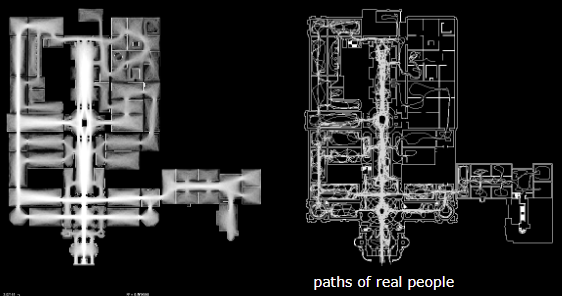
\includegraphics[width=\textwidth]{../assets/SingleVisualAgent1.png}
    \caption{Real People Data}
  \end{subfigure}
  \begin{subfigure}{0.49\textwidth}
    \centering
    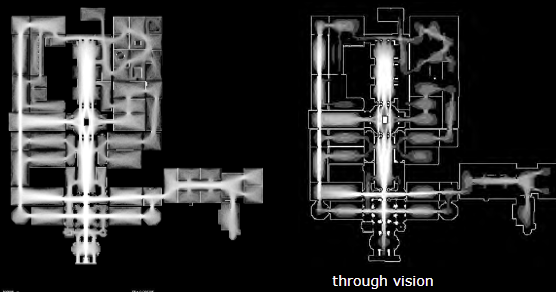
\includegraphics[width=\textwidth]{../assets/SingleVisualAgent2.png}
    \caption{Single Visual Agent Result}
  \end{subfigure}
\end{figure}

\subsection{Example: Groups of Interacting Agents}

\subsubsection{El Ferrol Bar Problem}

This problem was proposed by W. Brian Arthur.

Every Thursday night, a fixed population want to go have fun at the El Ferrol Bar, unless it's too crowded.

\begin{itemize}
  \item If less than 60\% of the population go to the bar, they will all have more fun than if they stayed home.
  \item If more than 60\% of the population go to the bar, they will all have less fun than if they stayed home.
\end{itemize}

Everyone must decide at the same time whether to go or not, with no knowledge of others' choices.

\textbf{Question: What is the rule of agents do decision in the computer experiment?}

Attendance rate maintains at around 60\%.

Agents can still make useful predictions with only partial information. This shows that we can still predict overall behaviour even when facing a complex system.

\section{Conclusion}

Two ways of thinking about design, and a system's outcome:

\begin{figure}[htbp]
  \centering
  \begin{subfigure}{0.49\textwidth}
    \centering
    \textbf{Emergent}
    \begin{itemize}
      \item Set up a series of rules and press `Go'
      \item Generates options /slash structures thought process
      \item Designer can rationalise processes and produce complexity
      \item examples:
      \begin{itemize}
        \item Animation /slash Parametric software
        \item Particle simulations
        \item Parametric CAD
        \item Shape grammars
        \item Cellular automata
      \end{itemize}
    \end{itemize}
  \end{subfigure}
  \begin{subfigure}{0.49\textwidth}
    \centering
    \textbf{Convergence}
    \begin{itemize}
      \item Makes simulation and analysis possible
      \item Allows designer to judge a complex design
      \item Respond to complex conditions, environments, etc.
      \item examples:
      \begin{itemize}
        \item Structural analysis FEM
        \item Light propagation /slash rendering algorithms
        \item Environmental simulation (e.g. ECOTECT)
        \item Acoustic simulation
        \item AI
      \end{itemize}
    \end{itemize}
  \end{subfigure}
\end{figure}

Divergence or convergence are both results of the dynamics of the system, i.e. the change between micro states, rather than the diversity of states themselves. They refer to a system being chaotic (if a small change in initial conditions leads to a very different outcome it is divergent) or stable (if the outcome is generally the same even from very different starting points it is convergent).

But this does also depend on how you are defining your macro states, which are how you view and measure your system. E.g. the weather is divergent but the climate is convergent.

\end{document}
